% Documento de exemplo usando o pacote customizado da UNEB

\documentclass[
	12pt,
	openright,		
	twoside,
	a4paper,
	english,
	brazil,
	]{abntex2}

\usepackage{uneb} 				% Customizacoes do ABNTEX para a UNEB
\usepackage{lmodern}			% Usa a fonte Latin Modern		
\usepackage[T1]{fontenc}		% Selecao de codigos de fonte.
\usepackage[utf8]{inputenc}		% Codificacao do documento (acentos)
\usepackage{lastpage}			% Usado pela Ficha catalografica
\usepackage{indentfirst}		% Indenta o primeiro paragrafo de cada secao.
\usepackage{color}				% Controle das cores
\usepackage{graphicx}			% Inclusao de graficos
\usepackage{microtype} 			% Melhorias de justificacao
\usepackage[alf,abnt-emphasize=bf]{abntex2cite}	% Citacoes padrao ABNT
\usepackage{lipsum}				% Geracao automatica de textos de exemplo
\usepackage{listings}			% Usa o pacote de Listings
\usepackage{color}				% Usa o pacote de cores
\definecolor{bluekeywords}{rgb}{0.13,0.13,1}
\definecolor{greencomments}{rgb}{0,0.5,0}
\definecolor{redstrings}{rgb}{0.9,0,0}

\lstset{language=[Sharp]C,
  showspaces=false,
  showtabs=false,
  breaklines=true,
  showstringspaces=false,
  breakatwhitespace=true,
  escapeinside={(*@}{@*)},
  frame=single,
  commentstyle=\color{greencomments},
  keywordstyle=\color{bluekeywords},
  stringstyle=\color{redstrings},
  basicstyle=\ttfamily\ABNTEXfontereduzida,
  inputencoding=utf8,
  morekeywords={*, :-}
}

% ----------------
% LISTA DE CÓDIGOS
% ----------------

% Altera o nome padrão do rótulo usado no comando \autoref{}
\renewcommand{\lstlistingname}{Código}

% Altera o rótulo a ser usando no elemento pré-textual "Lista de código"
\renewcommand{\lstlistlistingname}{Lista de códigos}

% Configura a "Lista de Códigos" conforme as regras da ABNT (para abnTeX2)
\begingroup\makeatletter
\let\newcounter\@gobble\let\setcounter\@gobbletwo
  \globaldefs\@ne \let\c@loldepth\@ne
  \newlistof{listings}{lol}{\lstlistlistingname}
  \newlistentry{lstlisting}{lol}{0}
\endgroup

\renewcommand{\cftlstlistingaftersnum}{\hfill--\hfill}

\let\oldlstlistoflistings\lstlistoflistings
\renewcommand{\lstlistoflistings}{%
   \begingroup%
   \let\oldnumberline\numberline%
   \renewcommand{\numberline}{\lstlistingname\space\oldnumberline}%
   \oldlstlistoflistings%
   \endgroup}

% Informacoes para capa e folha de rosto
\titulo{Título do Trabalho}
\autor{Autor do Trabalho}

\instituicao{Universidade do Estado da Bahia}
\departamento{Departamento de Ciências Exatas e da Terra}
\filiacao{Curso Superior Tecnológico em Jogos Digitais}
\orientador{Prof. Fulano de Tal}

\data{YYYY}
\local{Salvador-BA}

\preambulo{Texto apresentado ao Curso Superior Tecnológico de Jogos Digitais da Universidade do Estado da Bahia (UNEB), como requisito parcial para a obtenção do título de...
}
% --

% informacoes do PDF
\makeatletter
\hypersetup{
     	%pagebackref=true,
		pdftitle={\@title}, 
		pdfauthor={\@author},
    		pdfsubject={\imprimirpreambulo},
	    	pdfcreator={LaTeX with abnTeX2},
		pdfkeywords={abnt}{latex}{abntex}{abntex2}{trabalho acadêmico}, 
		bookmarksdepth=4
}
\makeatother
% --

\setlength{\parindent}{1.3cm} 	% Identacao da primeira linha
\setlength{\parskip}{0.2cm}  	% Espacamento entre um paragrafo e outro

\makeindex	% Sumario

% -------------------
% DOCUMENTO PRINCIPAL
% -------------------
\begin{document}

\selectlanguage{brazil}		% Idioma
\frenchspacing 				% Retira espaco extra entre as frases

% ----------------------
% ELEMENTOS PRÉ-TEXTUAIS
% ----------------------
\pretextual

\imprimircapa
\imprimirfolhaderosto

% Resumo em português
\setlength{\absparsep}{18pt} % ajusta o espaçamento dos parágrafos do resumo
\begin{resumo}

\lipsum[9-9]

 \textbf{Palavras-chave}: jogos digitais. games. game design.
\end{resumo}

% ---
% inserir lista de ilustrações
% ---
\pdfbookmark[0]{\listfigurename}{lof}
\listoffigures*
\cleardoublepage
% ---

% ---
% inserir lista de códigos
% ---
\pdfbookmark[0]{\lstlistlistingname}{lol}
\begin{KeepFromToc}
\lstlistoflistings
\end{KeepFromToc}
\cleardoublepage
% ---

% ---
% inserir lista de tabelas
% ---
\pdfbookmark[0]{\listtablename}{lot}
\listoftables*
\cleardoublepage
% ---

% ---
% inserir o sumario
% ---
\pdfbookmark[0]{\contentsname}{toc}
\tableofcontents*
\cleardoublepage
% ---

% ------------------
% ELEMENTOS TEXTUAIS
% ------------------
\textual

\chapter{Introdução}

\lipsum[1-2]

\section{Objetivos}

\lipsum[3-4]

\begin{alineas}
\item Objetivo 1...
\item Objetivo 2...
\item Objetivo 3...
\end{alineas} 

\section{Organização do Texto}

\lipsum[5-6]

\chapter{Fundamentação Teórica}

\lipsum[1-2]

\begin{citacao}
\lipsum[1]\cite[p. ~34]{Huizinga2014}
\end{citacao}

\section{Jogos Digitais}

De acordo com \citeonline{SalenZimmerman2012}, os jogos digitais...

\lipsum[4-7]

\section{Mundos Virtuais}

\lipsum[8-9]

A figura \ref{fig:kings-landing} representa \emph{King's Landing}, cenário da série \emph{Game of Thromes} reproduzido no Minecraft:

\begin{figure}[h]
	\caption{\emph{The King's Landing} no Minecraft}
	\center
	\label{fig:kings-landing}
	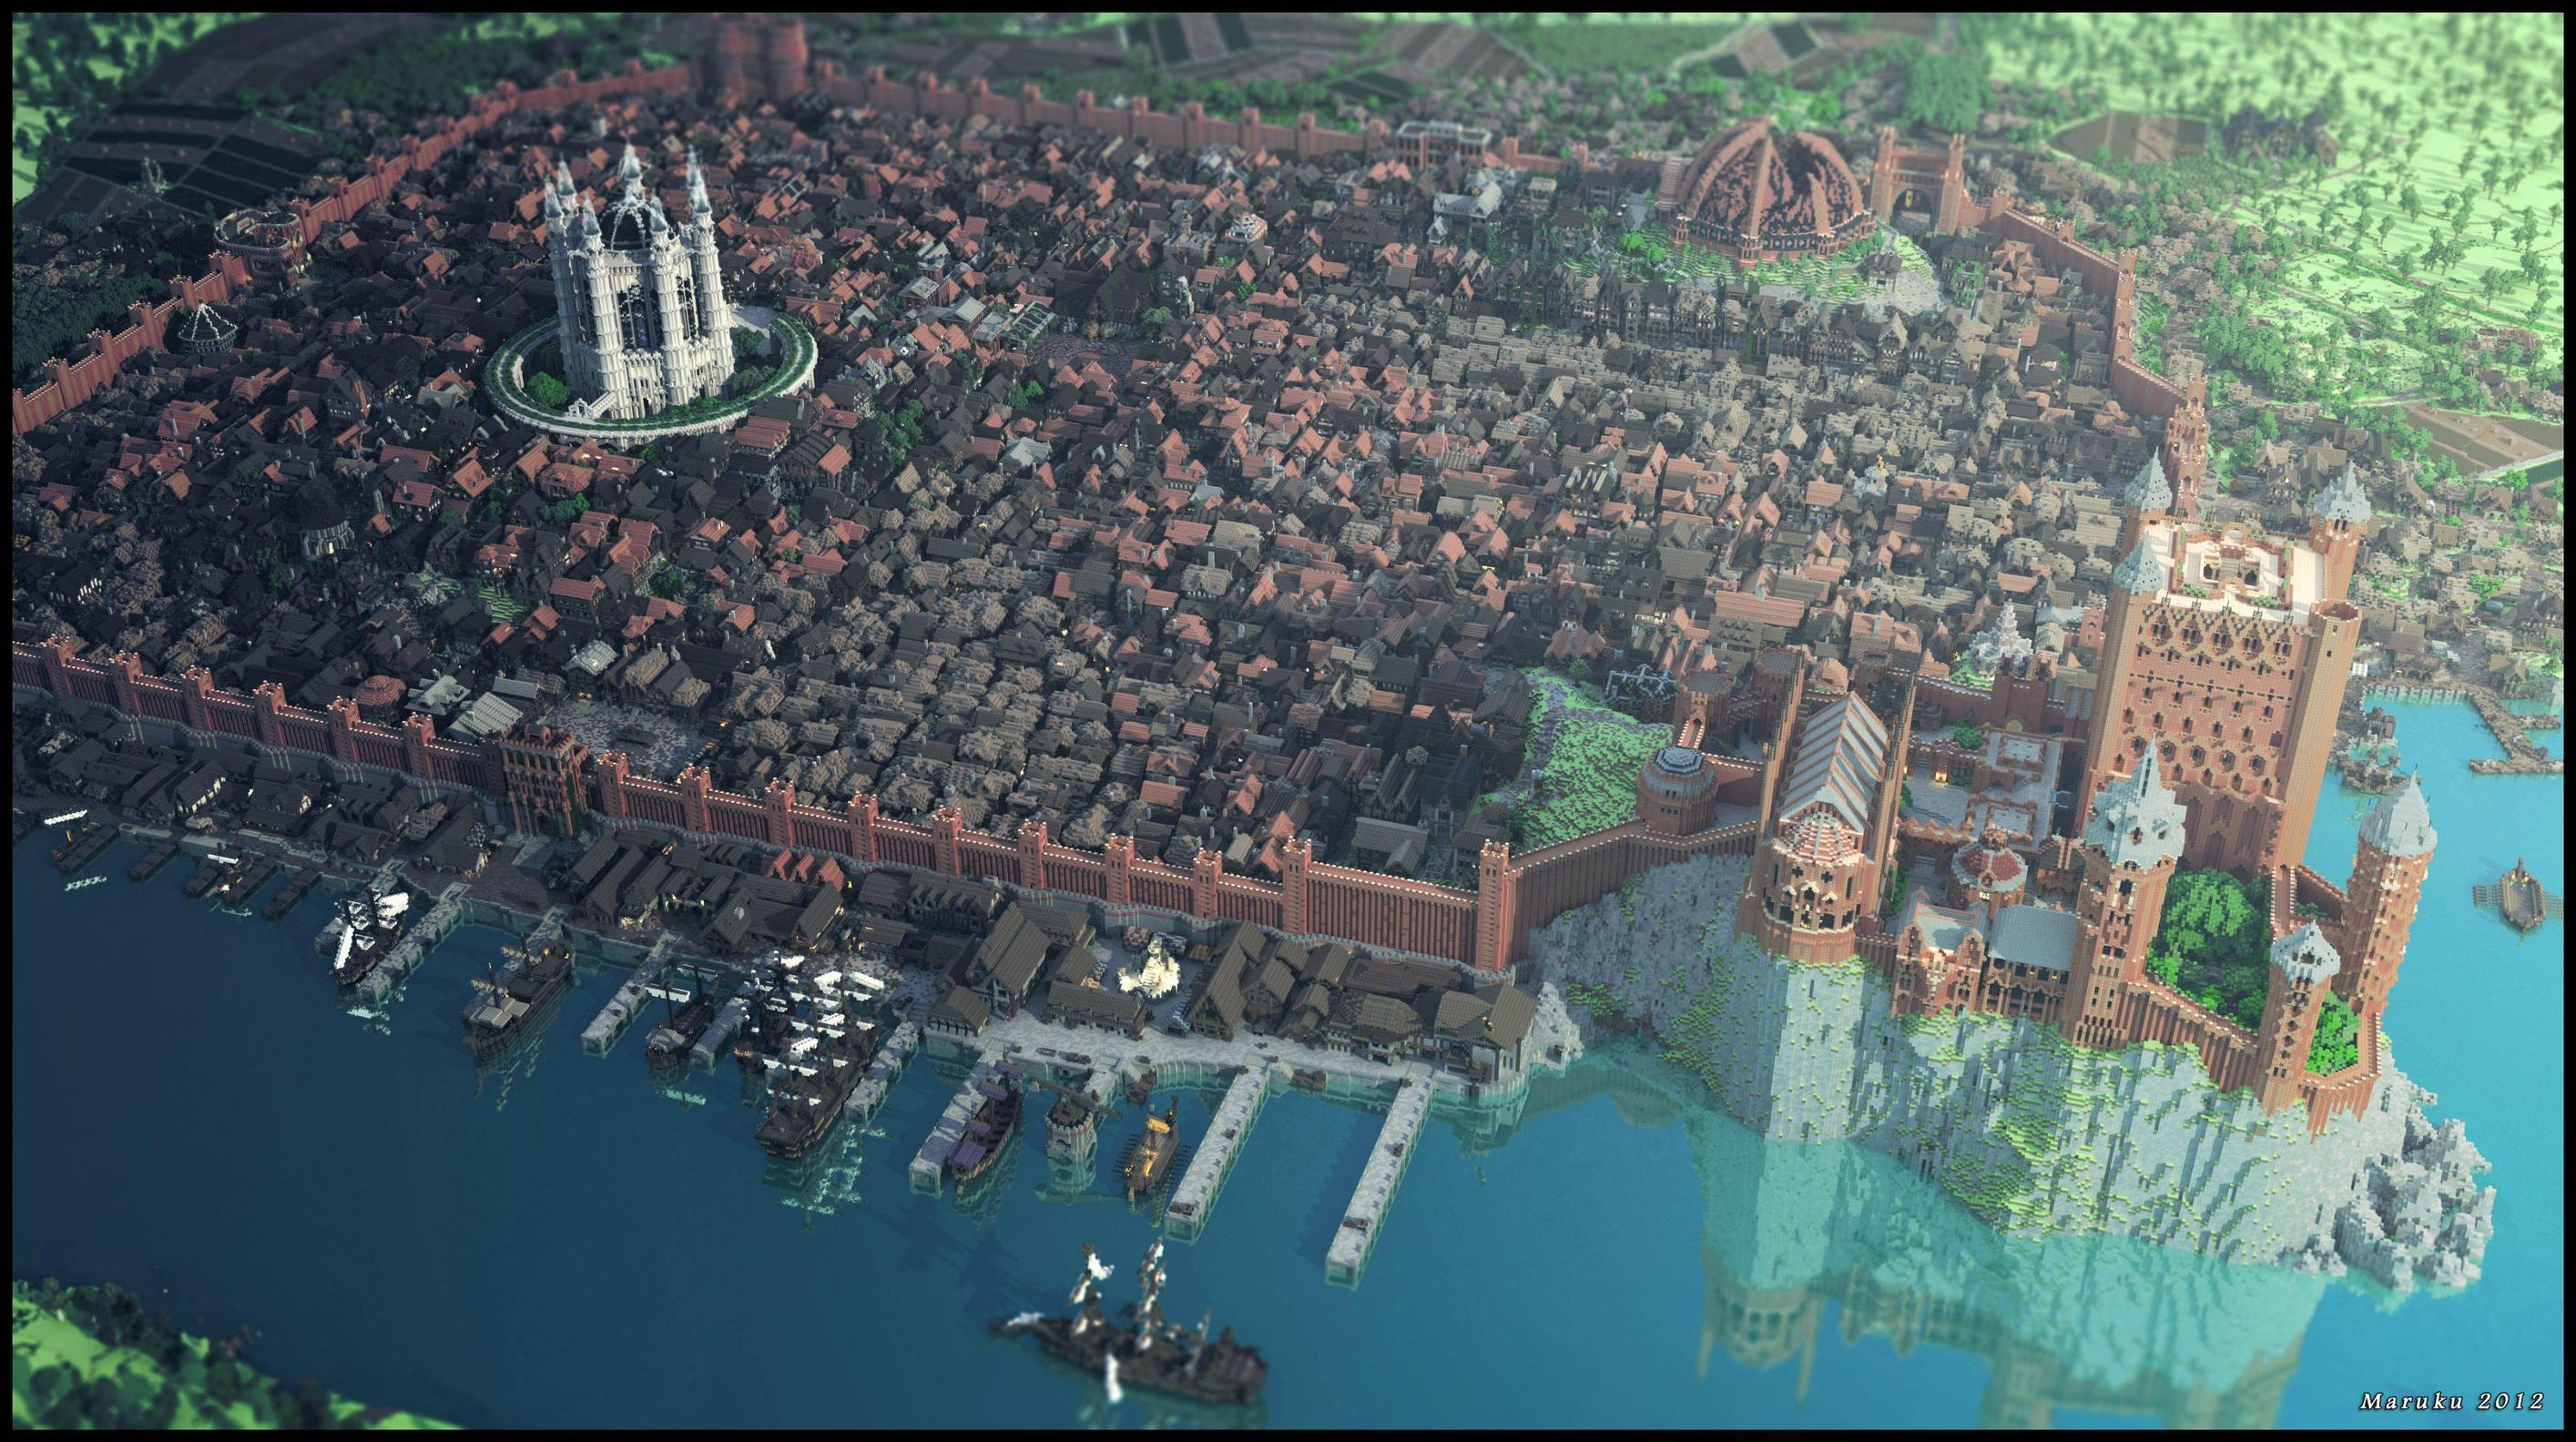
\includegraphics[scale=0.15]{fundamentacao/kings-landing.jpg}
	\fol{Imgur2013}
\end{figure}

\lipsum[10-12]


\chapter{Metodologia}

\lipsum[1-8]


\chapter{Análise dos Resultados}

\lipsum[1-2]

A tabela \ref{tab:newzoo} evidencia os jogos para PC mais populares em junho de 2019:

\begin{table}[h!] 
\caption{Jogos para PC mais Populares - Junho de 2019} 
\label{tab:newzoo}
	\begin{center} 
		\begin{tabular}{|c|l|} 
			\hline POSIÇÃO & JOGO \\
			\hline
			\hline 1 & League of Legends \\ 
			\hline 2 & Minecraft \\ 
			\hline 3 & Counter-Strike: Global Offensive \\
			\hline 4 & Hearthstone: Heroes of Warcraft \\
			\hline 5 & Fortnite \\						
			\hline
		\end{tabular} 
	\end{center}
	\legend{Fonte: \citeonline{Newzoo2019}} 
\end{table}

\lipsum[3-5]
\chapter{Conclusão}

\lipsum[1-4]


% ----------------------
% ELEMENTOS PÓS-TEXTUAIS
% ----------------------
\postextual

\bibliography{referencias}	% Referencias bibliograficas

\end{document}